\chapter{Objectieve beoordeling van een muziekstuk}
\label{hoofdstuk:OBM}
Om melodische transformaties te kunnen beoordelen is er nood aan een framework dat kan voorspellen of een gegeven melodie al dan niet goed klinkt. In dit hoofdstuk worden twee dergelijke modellen besproken die een bepaalde consonantiescore (maat voor het goed klinken van een muziekstuk) gaan toekennen aan een muziekstuk. 

Allereerst wordt een aanpak besproken die gebruik maakt van een artificieel neuraal netwerk \cite{book:ANN}. Deze methode is speciaal gemaakt voor het beoordelen van polyfone muziek, waarbij er meerdere noten tegelijk klinken. Polyfone muziek wordt in verdere hoofdstukken van deze masterproef niet meer besproken. Het eerste onderdeel van dit hoofdstuk zal bijgevolg dus weinig invloed hebben op het vervolg van de tekst. De methode is echter wel onderzocht geweest en leverde enkele interessante resultaten op waardoor de methode toch even in het kort vermeld wordt. 

Als tweede methode wordt een zogenaamd `RPK-Model' besproken dat gebaseerd is op een gelijknamig model uit \cite{book:musicAndProbability}. Dit model werkt op muziek met een enkele melodielijn en zal ook het model zijn dat als verificator gebruikt zal worden bij de experimenten in het vervolg van deze masterproef.

\section{Neuraal netwerk}
\label{OBM:NN}
In \cite{book:musimathics} wordt er een gedeelte gewijd aan het meten van de consonantie van akkoorden (samenklank van meerdere noten). Dit gebeurt kort samengevat door het trainen van een (feed forward) neuraal netwerk\cite{url:FFNN} op zogenaamde tweeklanken (twee noten die tegelijkertijd gespeeld worden). Het neuraal netwerk maakt dan de veralgemening naar hogere orde samenklanken. 

Het neuraal netwerk dat gemaakt werd als verificator bestond uit drie lagen. een invoerlaag, een uitvoerlaag en dan nog een verborgen laag. De invoerlaag bestond uit 12 neurons die elk voor een van de 12 verschillende noten staan. Twee noten die een octaaf uit elkaar liggen (en muziektechnisch dezelfde naam krijgen) zullen dus ook op eenzelfde neuron afgebeeld worden. Deze 12 input neurons krijgen een `1' als input wanneer er een noot in het akkoord zit die afgebeeld wordt op dat neuron. In het andere geval krijgt deze een `0' als input. Vervolgens komen we op een hidden layer terecht die volledig geconnecteerd is en uit 6 neurons bestaat. Tot slot komen we nog bij de output layer uit die uit slechts 1 neuron bestaat. Dit neuron gaat een getal tussen 0 en 1 teruggeven, hoe dichter het getal bij 1 ligt hoe zekerder het neuraal netwerk is dat het ingegeven akkoord consonant is. Hoe dichter bij 0 hoe zekerder het is dat het akkoord dissonant (tegengestelde van consonant) is. De lay-out van dit netwerk is weergegeven in figuur \ref{figuur:ANN}.\\

\def\layersep{2.5cm}
\def\doublelayersep{5.0cm}
\begin{figure}
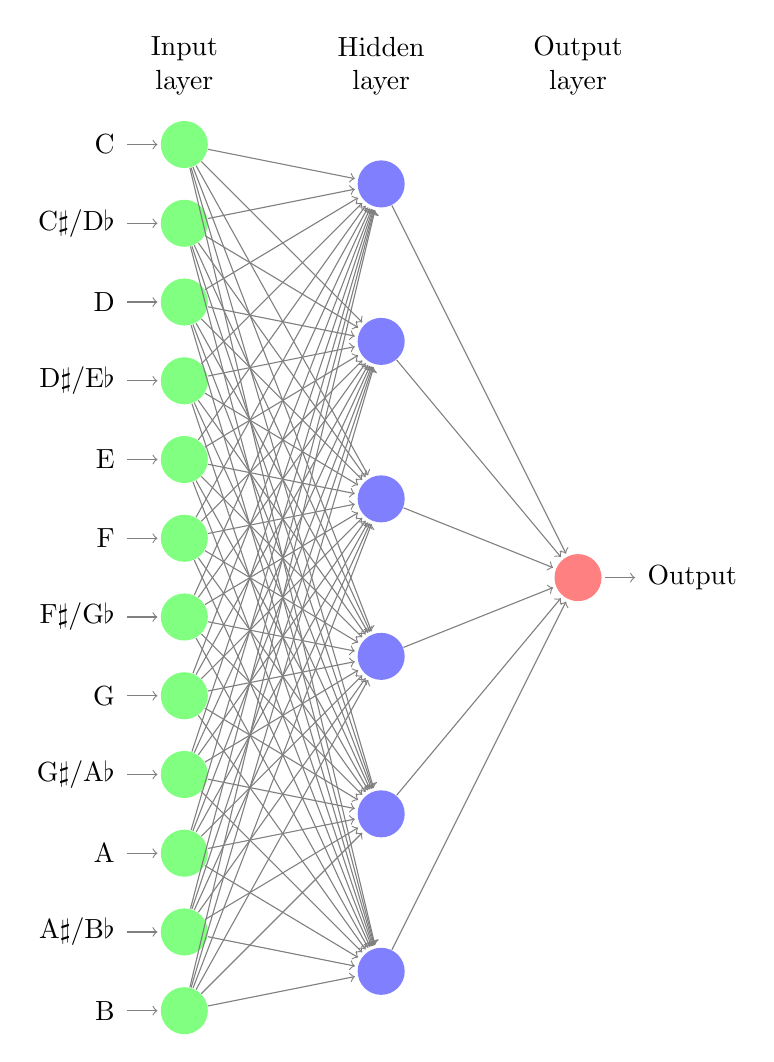
\begin{tikzpicture}[shorten >=1pt,->,draw=black!50, node distance=\layersep]
    \tikzstyle{every pin edge}=[<-,shorten <=1pt]
    \tikzstyle{neuron}=[circle,fill=black!25,minimum size=17pt,inner sep=0pt]
    \tikzstyle{input neuron}=[neuron, fill=green!50];
    \tikzstyle{output neuron}=[neuron, fill=red!50];
    \tikzstyle{hidden neuron}=[neuron, fill=blue!50];
    \tikzstyle{annot} = [text width=4em, text centered]

    % Draw the input layer nodes
    %\foreach \name / \y in {1,...,12}
    % This is the same as writing \foreach \name / \y in {1/1,2/2,3/3,4/4}
    %    \node[input neuron, pin=left:Input \#\y] (I-\name) at (0,-\y) {};
	\node[input neuron, pin=left:C] (I-1) at (0,-1) {};
	\node[input neuron, pin=left:C$\sharp$/D$\flat$] (I-2) at (0,-2) {};
	\node[input neuron, pin=left:D] (I-3) at (0,-3) {};
	\node[input neuron, pin=left:D$\sharp$/E$\flat$] (I-4) at (0,-4) {};
	\node[input neuron, pin=left:E] (I-5) at (0,-5) {};
	\node[input neuron, pin=left:F] (I-6) at (0,-6) {};
	\node[input neuron, pin=left:F$\sharp$/G$\flat$] (I-7) at (0,-7) {};
	\node[input neuron, pin=left:G] (I-8) at (0,-8) {};
	\node[input neuron, pin=left:G$\sharp$/A$\flat$] (I-9) at (0,-9) {};
	\node[input neuron, pin=left:A] (I-10) at (0,-10) {};
	\node[input neuron, pin=left:A$\sharp$/B$\flat$] (I-11) at (0,-11) {};
	\node[input neuron, pin=left:B] (I-12) at (0,-12) {};	
	
    % Draw the hidden layer nodes
    \foreach \name / \y in {1,...,6}
        \path[yshift=0.5cm]
            node[hidden neuron] (H-\name) at (\layersep,-\y*2 cm) {};

    % Draw the output layer node
    %\node[output neuron,pin={[pin edge={->}]right:Output}, right of=H-3] (O) {};
	\node[output neuron ,pin={[pin edge={->}]right:Output}] (O) at (\doublelayersep,-6.5 cm) {};

    % Connect every node in the input layer with every node in the
    % hidden layer.
    \foreach \source in {1,...,12}
        \foreach \dest in {1,...,6}
            \path (I-\source) edge (H-\dest);

    % Connect every node in the hidden layer with the output layer
    \foreach \source in {1,...,6}
        \path (H-\source) edge (O);

    % Annotate the layers
    \node[annot,above of=H-1, node distance=1.5cm] (hl) {Hidden layer};
    \node[annot,left of=hl] {Input layer};
    \node[annot,right of=hl] {Output layer};
\end{tikzpicture}
    \centering
    \caption{Neuraal netwerk met 12 input nodes (1 voor elke noot), 6 hidden nodes en 1 output node.}
    \label{figuur:ANN}
\end{figure}

Dit netwerk werd getraind op alle mogelijke tweeklanken gebruik makend van de \textit{backpropagation of error}-methode \cite{url:backpropagation}. Voor elke mogelijke tweeklank werd afhankelijk van de afstand (in halve tonen) tussen de twee noten bepaald of ze goed samen klinken of niet. Dit volgens de regels van de muziektheorie. Deze regels komen overeen met de verhoudingen van de frequenties van de twee invoernoten. Hoe kleiner de getallen in de vereenvoudigde breuk van de frequenties, hoe beter het akkoord klinkt. 

Na het trainen van het neuraal netwerk kan dit gebruikt worden om meerstemmige muziek te gaan beoordelen. Op elk tijdstip waarop er noten gespeeld worden kan men deze noten als input in het neuraal netwerk steken. De uitvoer van het netwerk geeft dan een maat voor de consonantie terug. Als we dit doen voor elk tijdstip in het muziekstuk waarop er noten gespeeld worden en we nemen dan het gemiddelde over al deze tijdstippen krijgen we een maat voor de gemiddelde consonantie van het hele muziekstuk.

Nadat het neuraal netwerk getraind werd, bleek het neuraal netwerk goed te generaliseren naar akkoorden met meer dan 2 noten. Dit wil zeggen dat akkoorden van meer dan twee noten die muziektheoretisch `goed' zouden moeten klinken ook door het netwerk als dusdanig beoordeeld werden. Het netwerk kon dus dienen als een soort van alternatieve voorstelling van de regels van de muziektheorie wat de samenklank van akkoorden betreft. Het probleem lag er echter in dat de klassieke werken van Bach en Mozart waarop getest werd zelf helemaal niet zo consonant waren als oorspronkelijk gedacht. Dit was in die mate het geval dat vaak tot een derde van de akkoorden in zo een stuk als dissonant (tegengestelde van consonant) bestempeld werden. Deze akkoorden blijken ook daadwerkelijk dissonant te zijn. Het is slechts door de context, de noten die net voor het akkoord gespeeld worden, dat deze akkoorden in die stukken toch niet als dissonant ervaren worden door de luisteraar. Het neuraal netwerk dat hier gebruikt werd houdt echter geen rekening met deze context. 

Dit leidt er toe dat dit neuraal netwerk niet gebruikt kan worden als verificator, aangezien zelfs muziekstukken van Bach en Mozart door de verificator niet als consonant herkend worden. Het is daarentegen wel nog maar eens een bevestiging van het genie van componisten als Bach en Mozart, de kunst ligt het niet in het volgen van de regels maar in het weten wanneer en hoe de regels gebroken mogen worden.

De broncode die geschreven werd voor het trainen van dit neuraal netwerk is beschikbaar in appendix \ref{Broncode:ANN}. Er zijn een aantal parameters die ingesteld kunnen worden in dit algoritme. Allereerst is er het aantal neuronen in de verborgen laag. Er kan ook een waarde voor de \textit{learning rate} opgegeven worden en dan zijn er nog twee parameters die een bias kunnen defini\"eren.

\section{Keuze tussen polyfone en monofone muziek}
\label{OBM:OMM}
In deze thesis wordt gewerkt met transformaties op een muziektheoretische manier (en dus niet fysisch met frequenties). Daarom wordt er gebruik gemaakt van muziekstukken die in het MusicXML\cite{url:musicxml} formaat beschikbaar zijn. Het nadeel van deze keuze is dat er slechts een beperkt aantal muziekstukken beschikbaar is. Dit in tegenstelling tot bijvoorbeeld het MIDI-formaat\cite{url:midi} waarbij dit niet het geval is. 

De polyfone(meerstemmige) muziek die beschikbaar is in het gewenste formaat bestaat eigenlijk bijna uitsluitend uit klassieke muziek. Verder is er ook nog een redelijk groot corpus beschikbaar van folkmuziek, het zogenaamde Essencorpus\cite{url:essen}. Deze muziek is wel monofoon (eenstemmig).

Aangezien de methode met het neuraal netwerk die beschreven staat in bovenstaand onderdeel niet voldoende werkte voor de meerstemmige stukken moest er een andere weg ingeslagen worden. Ofwel verder werken met meerstemmige muziek maar met een ander framework dat de context in rekening brengt. Ofwel de focus verleggen naar eenstemmige muziek. Gezien het grootste deel van de meerstemmige muziekstukken klassieke stukken zijn, is de keuze gemaakt om over te schakelen op eenstemmige muziek. Dit omdat de complexiteit van het aanpassen van muziekstukken met meerdere lijnen veel hoger is dan die van muziekstukken met slechts een instrument. Ook omdat klassieke muziekstukken veel delicater zijn om te behandelen dan stukken folkmuziek die enkel uit een melodielijn bestaan. Alle transformaties die zullen besproken worden in de rest van deze masterproef zullen dus ook uit een enkele melodielijn bestaan.

\section{RPK-model}
\label{OBM:RPK}
Aangezien er nood was aan een framework voor het beoordelen van muziekstukken van slechts een enkele melodielijn werd er uiteindelijk uitgekomen bij het zogenaamde RPK-model. Dit model wordt beschreven in \cite{book:musicAndProbability}. Het model dat besproken gaat worden in dit onderdeel en dus ook gebruikt werd in de rest van het onderzoek is gebaseerd op het model uit dit boek. Er werden een aantal vereenvoudigingen gedaan gebaseerd op extra data die beschikbaar is in het MusicXML formaat. Dit RPK-model gaat dus uit van een enkele lijn melodie (er wordt slechts een noot tegelijkertijd gespeeld). 

De waarschijnlijkheid van een bepaalde noot in een muziekstuk wordt gekenmerkt door de combinatie van 3 kenmerken waar het model naar genoemd is. 

Allereerst is er de zogenaamde \textit{range}, dit is de afwijking tot een centrale toonhoogte. Deze centrale toonhoogte is de noot die in het midden ligt van de distributie van alle noten uit alle muziekstukken van het beschikbare corpus. Globaal gezien hebben noten die dicht bij die centrum liggen een grotere waarschijnlijkheid tot voorkomen dan noten die verder van dit centrum verwijderd zijn. Dit wordt ge\"illustreerd in figuur \ref{figuur:range}, waarbij elke noot voorgesteld wordt door een geheel getal. De centrale C (do) heeft als waarde 60 gekregen. Een eenheid in deze schaal komt overeen met een halve toon, de volgende C krijgt dus als waarde 72 omdat het verschil tussen de deze twee noten 12 halve tonen is. 

Ook nog belangrijk om op te merken is dat in dit model een melodielijn als een opeenvolging van noten beschouwd wordt, zonder informatie over het ritme. Het ritme van een muziekstuk zal dus ook geen invloed hebben op de score die het RPK-model hieraan geeft. 

\begin{figure}[!ht]
  \centering
  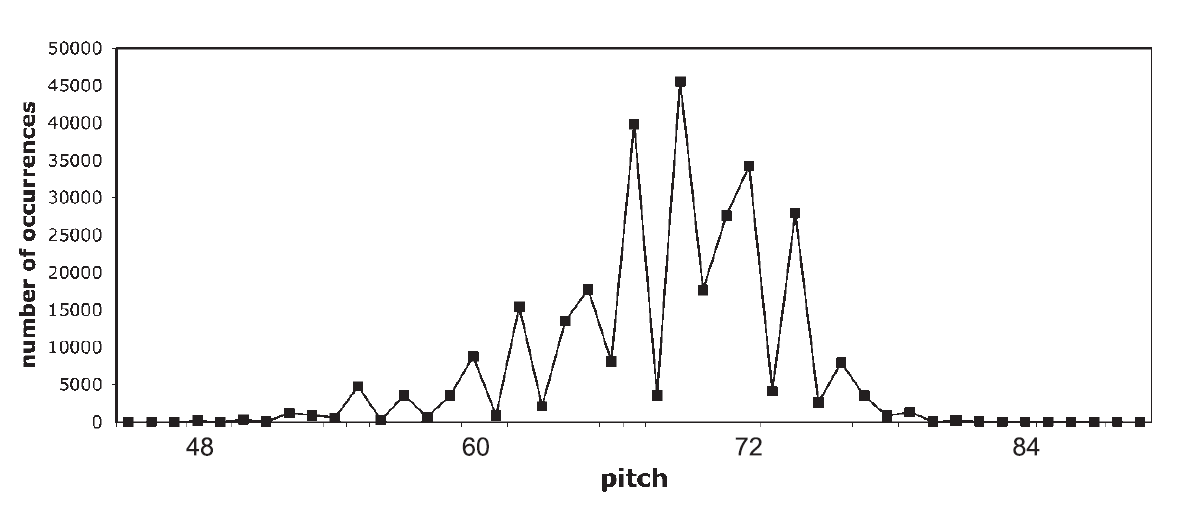
\includegraphics[width=0.75\textwidth]{2_Objectieve_Beoordeling/range}
  \caption{Distributie van alle noten in het Essencorpus.}
  \label{figuur:range}
\end{figure}

Verder is er ook nog de \textit{proximity}, dit heeft te maken met de relatieve afstand tot de voorgaande noot. Bepaalde groottes van sprongen zijn veel waarschijnlijker dan andere. Een sprong met een terts (3 of 4 halve tonen) of een kwint (7 halve tonen) komt bijvoorbeeld veel vaker voor dan een sprong van een sext(8 of 9 halve tonen). In het algemeen zijn kleine sprongen veel waarschijnlijker dan grotere. Figuur \ref{figuur:proximity} geeft de frequenties weer waarmee bepaalde intervallen tussen opeenvolgende noten voorkomen in het Essencorpus.

\begin{figure}[!ht]
  \centering
  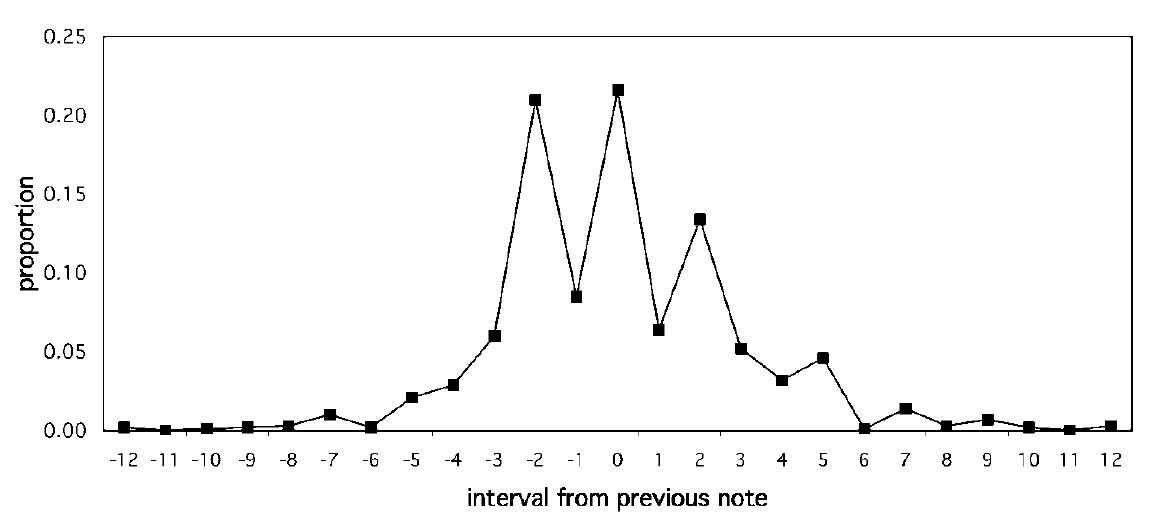
\includegraphics[width=0.75\textwidth]{2_Objectieve_Beoordeling/proximity}
  \caption{Proporties van voorkomen van alle intervallen van opeenvolgende noten in het Essencorpus.}
  \label{figuur:proximity}
\end{figure}

Ten slotte wordt er ook nog rekening gehouden met de \textit{key}, ofwel de toonaard van het muziekstuk. Afhankelijk van de toonaard zijn bepaalde noten waarschijnlijker om voor te komen dan andere. Zo is de grondtoon van een toonladder bijvoorbeeld altijd sterk aanwezig terwijl de noot die een halve toon hoger ligt quasi nooit zal voorkomen in het muziekstuk. Ook is er een verschil in profiel tussen majeur en mineur toonaarden, hier wordt ook rekening mee gehouden. Dit wordt ook ge\"illustreerd in figuren \ref{figuur:key_major} en \ref{figuur:key_minor} die respectievelijk voor stukken die in grote en kleine toonaarden staan de distributies van noten uit het Essencorpus weergeeft. 

\begin{figure}[!ht]
  \centering
  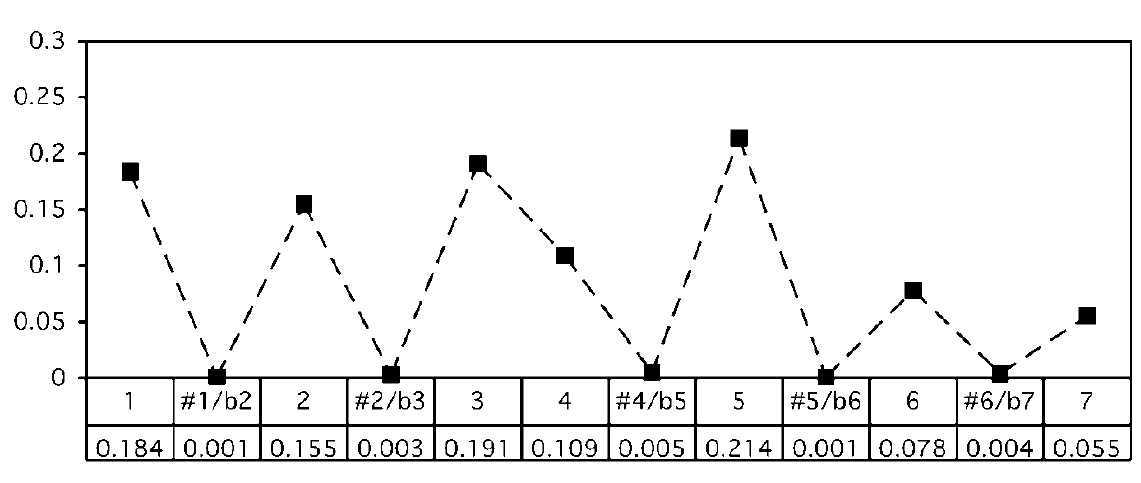
\includegraphics[width=0.75\textwidth]{2_Objectieve_Beoordeling/key_major}
  \caption{Proporties van voorkomen in het Essencorpus van nootfuncties in grote toonladder.}
  \label{figuur:key_major}
\end{figure}

\begin{figure}[!ht]
  \centering
  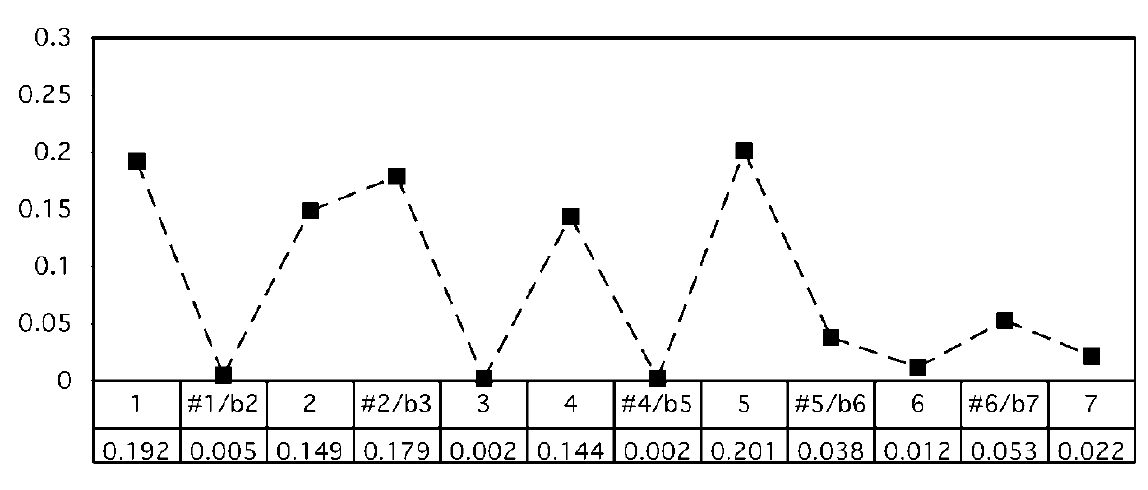
\includegraphics[width=0.75\textwidth]{2_Objectieve_Beoordeling/key_minor}
  \caption{Proporties van voorkomen in het Essencorpus van nootfuncties in kleine toonladder.}
  \label{figuur:key_minor}
\end{figure}

De \textit{range}- en \textit{proximity}-waarden worden gemodelleerd door een normaal verdeling rond respectievelijk de centrale en de vorige noot uit het muziekstuk. De \textit{key}-waarde van een noot wordt bepaald aan de hand van de frequentie van voorkomen van zijn nootfunctie in alle muziekstukken van het corpus.

\subsubsection{Bepaling score van een volledige melodielijn}
Nu kan voor elke noot in een melodielijn bepaald worden wat zijn waarschijnlijkheid is. Dit gebeurt door het product te nemen van zijn drie verschillende probabiliteitsscores (\textit{range}, \textit{proximity} en \textit{key}) en dit te normaliseren over alle mogelijke toonhoogtes. De score van een volledige melodielijn staat dan gelijk aan de gemiddelde score over al zijn noten. De score van een melodielijn geeft dus weer wat de gemiddelde waarschijnlijkheid is van een noot in die melodielijn volgens het RPK-model. 

De score van een melodielijn kan berekend worden door het product te nemen van de scores van elke noot in het stuk en hier dan het meetkundig gemiddelde van te nemen. Aangezien dit product kan leiden tot zeer kleine waarden voor de waarschijnlijkheid wordt in de plaats daarvan gerekend met de logaritmes van deze probabiliteiten. De probabiliteitsscore van een noot wordt dus voorgesteld door het logaritme van zijn echte probabiliteit. De score van een volledige melodielijn is nu dus het rekenkundig gemiddelde van de individuele scores van alle noten in het muziekstuk. Dit is computationeel interessanter. 

De broncode die gebruikt werd om deze scores te berekenen wordt weergegeven in appendix \ref{Broncode:RPK}. De score die in deze code berekend wordt voor een muziekstuk is de som van de logaritmen van de probabiliteiten van alle noten in het muziekstuk. Door deze waarde te delen door het aantal noten in het muziekstuk kan een gemiddeld logaritme van de probabiliteit bekomen worden.

\subsubsection{Beoordeling van een muziekstuk}
Men zou snel kunnen stellen dat voor het beoordelen van een muziekstuk met het RPK-model er gewoon gekeken zal worden naar de score die het model geeft aan dat stuk en dat een hogere score dan logischerwijs overeenkomt met een (theoretisch gezien) beter muziekstuk. Er moet echter ook rekening gehouden worden met de beperkingen van het RPK-model. 

Aangezien dit model afhankelijk is van de drie besproken parameters zal een ideale melodielijn voor dit model bestaan uit een opeenvolging van noten van telkens dezelfde toonhoogte (zodat de afstand tot de vorige noot telkens 0 is), waarvan deze noot zeer waarschijnlijk is in de toonaard en dicht bij de centrale toonhoogte ligt. Het RPK-model geeft dus hoge scores aan stukken die zich dicht rond de centrale noot afspelen en kleine sprongen vertonen tussen opeenvolgende noten. Dit zijn echter niet de meest interessante muziekstukken om naar te luisteren. 

Vandaar dat bij het beoordelen van een transformatie er gaat gekeken worden naar het verschil in scores tussen het originele muziekstuk en zijn getransformeerde versie. Hierbij zal een transformatie als beter bestempeld worden dan een andere wanneer hij gemiddeld gezien minder afwijking van score oplevert tussen de getransformeerde melodie en het originele muziekstuk. De reden dat dit zo gebeurt is omdat de originele stukken telkens verondersteld worden van goede kwaliteit te zijn. 

Een sterke verbetering in score zou dan betekenen dat het stuk waarschijnlijk minder interessant is geworden (minder grote sprongen, meer voorspelbaarheid). Een sterke verlaging van de score zou betekenen dat het stuk te onvoorspelbaar geworden is en een grotere kans heeft om als frustrerend ervaren te worden door de luisteraar. Vandaar dat de score van het originele stuk telkens als een soort van `gouden verhouding' zal bekeken worden horende bij het ritme van dat stuk (dat onveranderd zal blijven na melodische transformatie) tussen voorspelbaarheid en verrassing.  

%%% Local Variables: 
%%% mode: latex
%%% TeX-master: "masterproef"
%%% End: 
